\begin{frame}{Interesting results - Acceptability Theorem }
    \pause
    \begin{minipage}[t]{0.45\linewidth}
    \vspace{-2.5em}
    \begin{theorem}[Reducing Exhaustion-reflection to Exhaustion-reflection for Cubes]
        We show that to prove that a function $f:\Reals^n \to\Reals^m$ is exhaustion-reflecting, it suffices to show that we can compute, for any rational open $m$-cube $Q$, an open exhaustion for $f^{-1}(Q)$.
    \end{theorem}
    \pause
    \vspace{-1 em}
    \begin{theorem}[Reducing Exhaustion-reflection for Cubes to a Decision Procedure]
        Let $U \subseteq \Reals^2$ be an open set. If there is a recursive function
        \vspace{-1em}
        \[
        \vspace{-1em}
        \mathsf{in}_U:\Rationals^{2} \times \Rationals^2\to \Bools
        \] 
        % \vspace{-1em}
        taking $(a_1,b_1, a_2, b_2)$ as inputs and deciding whether the closed rational $2$-cube 
        \vspace{-1em}
        \[
        [a_1,b_1] \times [a_2, b_2]
        \vspace{-1em}
        \]
        is completely contained in $U$, then $U$ has an effective open exhaustion.
    \end{theorem}

    \end{minipage}
    \begin{minipage}[t]{0.54\linewidth}
        \center
        \pause
        \vspace{-1em}
        \color{MidnightBlue}
        \textbf{The process of building an effective open exhaustion}
        \vspace{-1em}
        \begin{flushright}
            \pause
            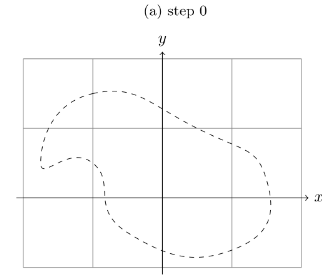
\includegraphics[width=0.48\linewidth]{tikz/step0.png}
            \pause
            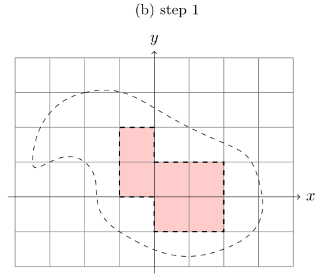
\includegraphics[width=0.48\linewidth]{tikz/step1.png}
            \pause
            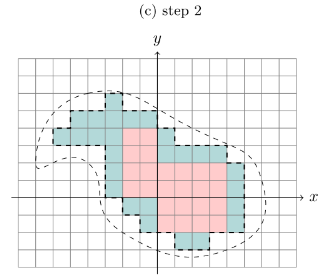
\includegraphics[width=0.48\linewidth]{tikz/step2.png}
            \pause
            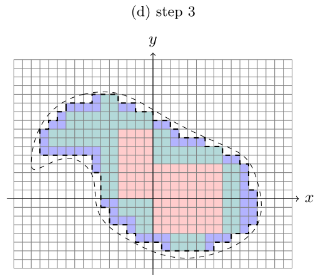
\includegraphics[width=0.48\linewidth]{tikz/step3.png}
        \end{flushright}
    \end{minipage}
\end{frame}